\documentclass{article}
\usepackage{fullpage}
\usepackage[utf8]{inputenc}

\title{Pro Features Demo}
\author{Courtney Gibbons}
\date{July 2020}

\usepackage{natbib}
\usepackage{graphicx}

\begin{document}

\maketitle

\section{Introduction}
There is a theory which states that if ever anyone discovers exactly what the Universe is for and why it is here, it will instantly disappear and be replaced by something even more bizarre and inexplicable.
There is another theory which states that this has already happened.

\noindent{\Huge  go ahead and edit this project however you like!}

Did it record that I deleted "please"?

\noindent{\tiny How small is "tiny", I wonder?}

\bigskip

Click on the ``Review'' tab (top right) to see the edits people have made.

Click ``Chat'' to see what people are saying about the document.  Click ``History'' to see versions of the document.


\bigskip

\hrule


\begin{figure}[h!]
\centering
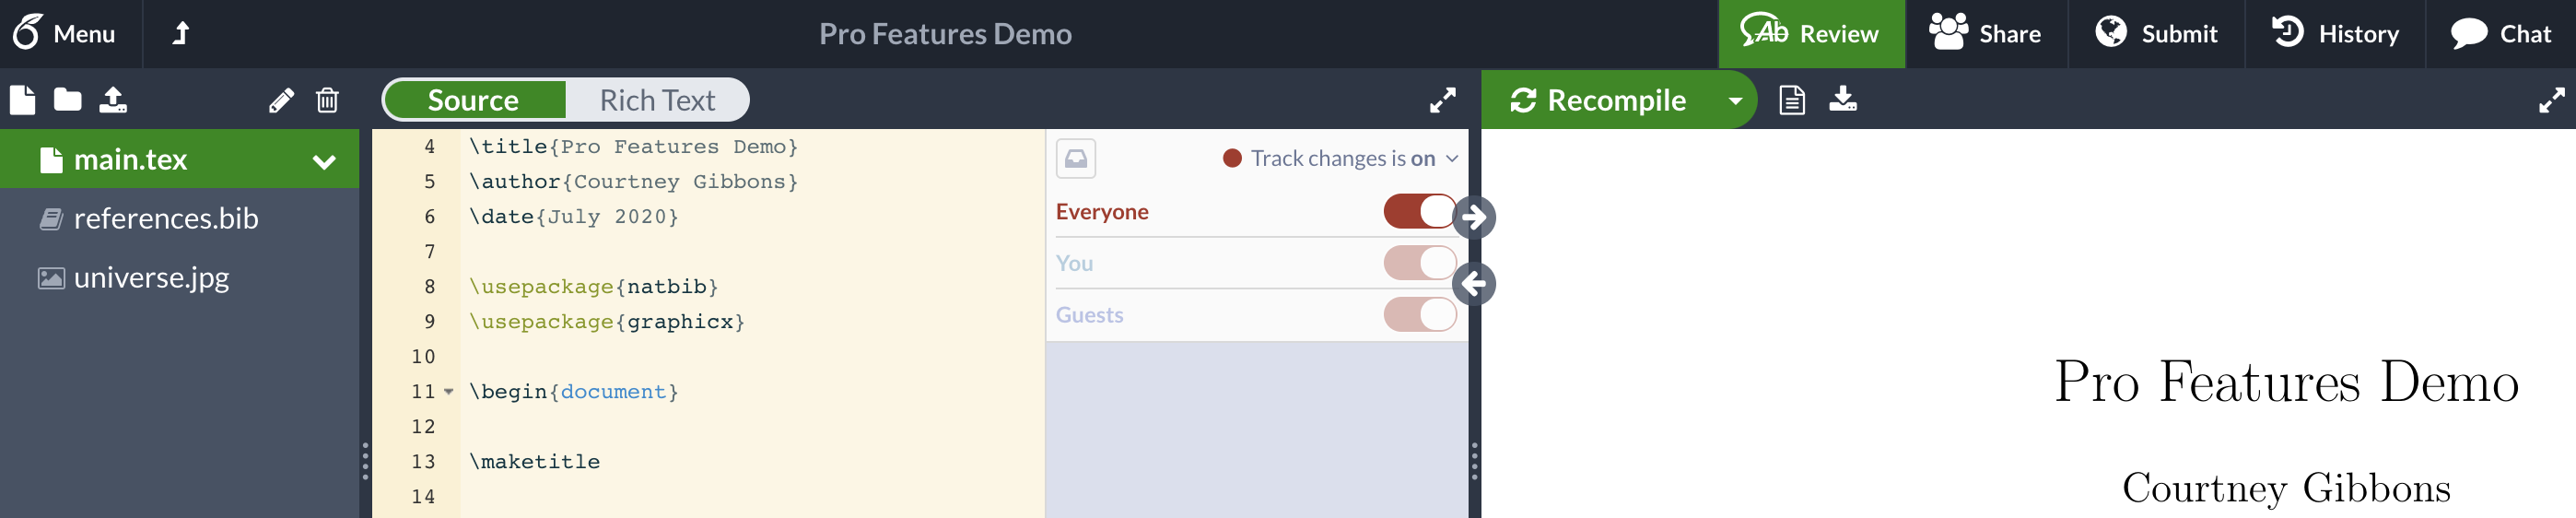
\includegraphics[width=.9 \textwidth]{Screenshot 2020-07-27 12.16.31.png}
\caption{The menu bar}
\label{fig:universe}
\end{figure}

\section{Conclusion}
``I always thought something was fundamentally wrong with the universe'' \citep{adams1995hitchhiker}

\bibliographystyle{plain}
\bibliography{references}
\end{document}
